% VLDB template using acmart
\documentclass[sigconf, nonacm]{acmart}
\usepackage{pvldb}

\usepackage{amsmath,amsfonts}
\usepackage{algorithm}
\usepackage{algorithmic}
\usepackage{graphicx}
\graphicspath{{figures/}}
\usepackage{textcomp}
\usepackage{xcolor}
\usepackage{booktabs}
\usepackage{multirow}
\usepackage{xspace}
\usepackage{tikz}
\usetikzlibrary{arrows.meta, positioning, fit, backgrounds, shapes.geometric}
\settopmatter{printacmref=false}

\newcommand{\DynaSCSH}{\textsc{DYNASCSH}\xspace}
\newcommand{\mtindex}{\textsc{MT-INDEX}\xspace}
\newcommand{\qratio}{\text{$Q$-Ratio}\xspace}

%% PVLDB metadata. Replace DOI/pages after acceptance.
\renewcommand\vldbdoi{XX.XX/XXX.XX}
\renewcommand\vldbpages{XXX-XXX}
\renewcommand\vldbvolume{20}
\renewcommand\vldbissue{1}
\renewcommand\vldbyear{2027}
\renewcommand\vldbtitle{Dynamic Size-Constrained Community Search over Evolving Heterogeneous Information Networks}
\renewcommand\vldbavailabilityurl{https://github.com/wzw7234895/DynaSCSH}

\begin{document}

\title[Dynamic Size-Constrained Community Search]{Dynamic Size-Constrained Community Search over\texorpdfstring{\\}{ }Evolving Heterogeneous Information Networks}

\author{Zhiwei Wang}
\affiliation{%
  \institution{Dalian Maritime University}
  \city{Dalian}
  \country{China}
}
\email{wzw7234895@gmail.com}

\begin{abstract}
Heterogeneous information networks (HINs) model typed entities and relations. Community search on HINs identifies cohesive subgraphs containing a query node, with applications in recommendation, fraud detection, and expert finding. While Zhang et al. recently formalized the size-constrained variant and proved it NP-hard, their solution is inherently static---recomputing communities from scratch whenever the graph changes. Real-world HINs are dynamic: new collaborations form, products are purchased, and relationships evolve continuously.

We propose \DynaSCSH, a dynamic framework for maintaining size-constrained $(k,\mathcal{P})$-truss communities under projected source-edge insertions and deletions. \DynaSCSH combines three components: (1) a Meta-Path Triangle Index (\mtindex) storing $O(|E|)$ integer support counts and updating all co-triangle edge supports affected by a source-edge change, (2) an internal support cache that makes community validation independent of the full graph size, and (3) a localized repair mechanism with bounded-hop candidate search that validates support, size, query containment, and triangle connectivity before returning a repaired community.

Experiments on 22 fixed-query synthetic DBLP configurations and a hybrid Planted Community Benchmark (26,850 nodes, 128,227 edges) demonstrate the properties of incremental maintenance. On insertion-only streams, \DynaSCSH preserves community identity exactly (Jaccard=1.000, avg.\ \qratio=1.000, avg.\ 3,824$\times$ speedup vs.\ static recompute). Deletion and mixed streams introduce natural divergence: deletion Jaccard spans 0.36--0.54 (\qratio=0.89--0.92), reflecting the inherent difficulty of maintaining a fixed-size community under edge removal. The hybrid benchmark confirms scalability to 128K-edge graphs (random updates $<$1\,ms, 5,900--10,700$\times$ speedup) and demonstrates localized repair success (10/30 targeted community-edge deletions repaired at $k$=2). Strict invariant checking (support, size, query containment, triangle connectivity) makes fallback recomputation explicit when local repair cannot certify validity.
\end{abstract}

\maketitle

\vldbtopmatter

\section{Introduction}

Heterogeneous information networks (HINs) model real-world systems with multiple node and edge types, such as bibliographic networks (authors, papers, venues), e-commerce platforms (users, products, categories), and knowledge graphs (entities, relations, types). Community search---finding a cohesive subgraph containing a given query node---is a fundamental operation over HINs, with applications in expert recommendation, fraud ring detection, and product suggestion~\cite{zhang2025scsh,sach2024icde}.

Zhang et al.~\cite{zhang2025scsh} recently formalized the \emph{size-constrained} community search problem over HINs (SCSH), which seeks a community of exactly $s$ nodes maximizing the $(k,\mathcal{P})$-truss cohesiveness metric. They proved the problem NP-hard and proposed exact Branch \& Bound algorithms with polynomial-time heuristics. However, their solution is fundamentally \emph{static}: any change to the graph requires recomputing the community from scratch.

This static assumption is at odds with reality. HINs evolve continuously: authors publish new papers, customers purchase additional products, and entities acquire new relationships. Recomputing communities from scratch after each update incurs substantial latency---in our reported synthetic and hybrid runs, the fixed-query greedy baseline averages roughly 390--950~ms per checkpointed recomputation. For applications such as interactive expert recommendation or fraud monitoring where updates arrive at sub-second intervals, this per-update cost cannot be amortized: the recomputation latency exceeds the inter-update gap, making static recomputation a throughput bottleneck even at modest graph scales.

The natural question is: \emph{Can we maintain size-constrained communities incrementally as the graph evolves, avoiding the cost of full recomputation?}

This paper answers affirmatively with \textbf{\DynaSCSH}, the first dynamic size-constrained community search framework for evolving HINs. \DynaSCSH combines three novel components:

\begin{enumerate}
\item \textbf{Meta-Path Triangle Index (\mtindex):} A count-based $O(|E|)$ index tracking meta-path triangle participation per edge, updated in $O(d_{\mathcal{P}}(u)\cdot d_{\mathcal{P}}(v))$ time per edge change. Triangle structures are resolved on-demand during cascading truss collapse rather than pre-materialized, avoiding the $O(|E|\cdot d_{\max}^2)$ memory explosion of explicit triangle storage.

\item \textbf{Internal Support Cache:} A running dictionary of $(k,\mathcal{P})$-truss support counts for edges \emph{within} the maintained community, computed strictly over the induced subgraph. This makes validation independent of the full graph size and exposes the common fast path where a projected-edge update does not touch the maintained community.

\item \textbf{Localized Repair with Validated Fallback:} When community edges are deleted, \DynaSCSH searches for replacement nodes within a bounded hop radius. A repaired community is returned only after checking size, original query containment, internal support, and triangle connectivity. If no candidate passes validation, \DynaSCSH falls back to the same fixed-query greedy recomputation used by the static baseline.
\end{enumerate}

We evaluate \DynaSCSH in two evidence-backed settings: 22 fixed-query synthetic DBLP configurations and a separate 26,850-node hybrid benchmark combining real DBLP topology with planted dense communities.

\textbf{Key findings (post-fix, fixed-query baseline, 22 configurations):}
\begin{itemize}
\item \textbf{Insertion streams:} With a fixed query node, \DynaSCSH preserves structure exactly (Jaccard=1.000 in all 17 insertion runs) and keeps quality at parity on average (\qratio=1.000), with 3,824$\times$ average speedup.
\item \textbf{Deletion streams:} Deletions diverge naturally: Jaccard 0.36--0.54 and \qratio 0.89--0.92. They still average 2,188$\times$ speedup; D1 drops to 1.4$\times$ when fallback dominates.
\item \textbf{Invariant-checked repair:} Local repair is accepted only after support, size, query containment, and triangle connectivity checks; otherwise the framework falls back to fixed-query greedy recomputation.
\item \textbf{Planted Community Benchmark:} On a 26,850-node hybrid graph (real DBLP topology + 40 planted dense communities), \DynaSCSH achieves 5,900--10,700$\times$ speedup under the fixed-query baseline, preserves community identity (Jaccard=1.000 across the reported hybrid insertion/deletion streams), and repairs 10/30 targeted community-edge deletions at $k$=2.
\end{itemize}

\begin{figure*}[htbp]
\centering
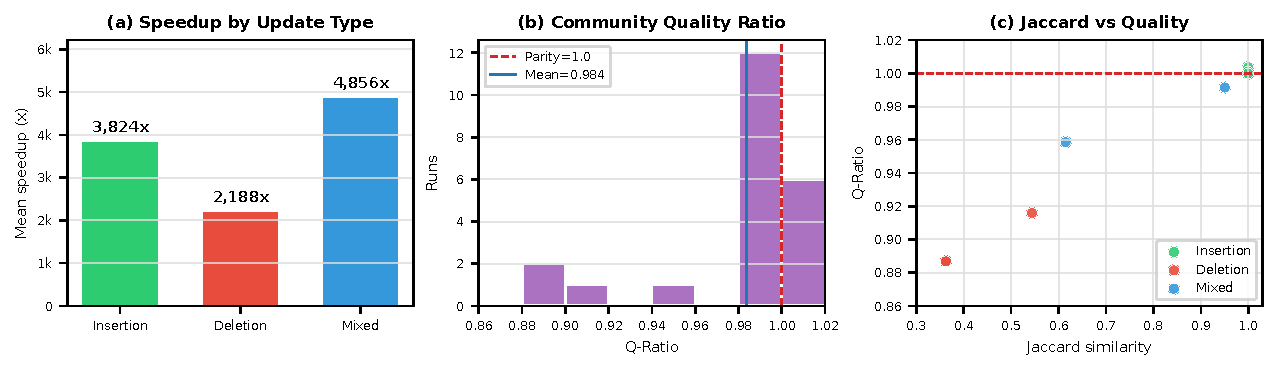
\includegraphics[width=.78\textwidth]{figures/fig_teaser.pdf}
\caption{Overview under the fixed-query baseline. (a) Speedups by update type on the synthetic benchmark. (b) \qratio distribution across 22 configurations. (c) Jaccard vs.\ \qratio, showing that structural overlap and score can diverge even when dynamic and static methods use the same query.}
\Description{Three-panel teaser showing speedups, quality-ratio distribution, and Jaccard versus Q-Ratio under the fixed-query baseline.}
\label{fig:teaser}
\end{figure*}

\section{Related Work}

We survey work in three areas: community search in HINs, dynamic graph algorithms, and size-constrained subgraph mining.

\subsection{Community Search in HINs}

Community search over HINs has attracted significant attention. Zhang et al.~\cite{zhang2025scsh} formalized the size-constrained variant (SCSH) using the $(k,\mathcal{P})$-truss model, proved NP-hardness, and proposed Branch \& Bound algorithms (ESG and NSG). Our work extends theirs to the dynamic setting.

Several recent ICDE and PVLDB publications address related problems: SACH~\cite{sach2024icde} introduces significant-attributed community search with segment-based meta-path expansion; a self-training GNN-based approach~\cite{chen2024icde} tackles the MK (Most-likely $K$-sized) community search problem on attributed HINs; Wang et al.~\cite{wang2025pvldb} propose the Structurally Similar Community (SSC) model with four vertex roles. Tang et al.~\cite{tang2025pvldb} address temporal HIN community search with the $(k,T_q,\mathcal{P},\delta)$-core model. Han et al.~\cite{han2025vldb} propose the $(\tau,\rho)$-camp model unifying triangle and quadrilateral semantics. None of these works handle \emph{size-constrained} community maintenance under dynamic edge updates.

\subsection{Dynamic Graph Algorithms}

Dynamic community search has been studied primarily over homogeneous graphs. CS-DAHIN~\cite{song2024tkde} addresses community search over dynamic attributed HINs but does \emph{not} incorporate size constraints. DAHIN-INCE~\cite{cao2025bdsc} proposes incremental learning for dynamic attributed HINs using knowledge distillation. For streaming graphs, Liao et al.~\cite{liao2024pvldb} propose D-truss maintenance over directed streams, and Zhang et al.~\cite{zhang2024arxiv} address community detection over streaming bipartite networks. Our work fills the gap between these dynamic (but unconstrained) methods and Zhang et al.'s static (but size-constrained) framework.

\subsection{Size-Constrained Subgraph Mining}

Beyond HINs, size-constrained dense subgraph discovery has been studied on homogeneous graphs. CCSS~\cite{he2024eswa} proposes conductance-based community search with size constraints. The densest-$k$ subgraph problem has a rich theoretical literature. Our $(k,\mathcal{P})$-truss model inherits its structural guarantees from this lineage while adding HIN-specific meta-path semantics.

\subsection{Positioning}

To our knowledge, \DynaSCSH is the \emph{first} framework to simultaneously address: (1) size constraints on community cardinality, (2) heterogeneous meta-path semantics, and (3) dynamic edge updates with incremental maintenance. The closest prior works each address at most two of these three dimensions.

\section{Preliminaries}

We briefly review the HIN model, the $(k,\mathcal{P})$-truss community definition, and the static SCSH problem. Table~\ref{tab:notation} summarizes the key notation used throughout the paper.

\subsection{Heterogeneous Information Networks}

A heterogeneous information network (HIN) is a typed graph $\mathcal{G} = (V,E,\phi,\psi)$. Here $V$ and $E$ are nodes and edges, $\phi:V\rightarrow\mathcal{T}_V$ maps nodes to types, and $\psi:E\rightarrow\mathcal{T}_E$ maps edges to types, with multiple node or edge types. A \emph{meta-path} $\mathcal{P} = (T_1 \xrightarrow{R_1} T_2 \xrightarrow{R_2} \cdots \xrightarrow{R_{l-1}} T_l)$ specifies a composite relation between node types. For example, in a bibliographic HIN with Author (A), Paper (P), and Venue (V) types, the meta-path APA denotes co-authorship via shared papers.

\subsection[The k,P-truss Model]{The $(k,\mathcal{P})$-truss Model}

The $(k,\mathcal{P})$-truss~\cite{zhang2025scsh} generalizes the classical $k$-truss to HINs. For a symmetric meta-path $\mathcal{P}$ (where $T_1 = T_l$) and an edge $(u,v)$ whose endpoints both have type $T_1$, the \emph{meta-path triangle support} is:

\begin{equation}
\sigma_{\mathcal{P}}(u,v) = \big|\{ w \in V \mid (u,v,w) \text{ form a $\mathcal{P}$-triangle} \}\big|
\label{eq:support}
\end{equation}

where a $\mathcal{P}$-triangle requires that all three pairwise edges exist and that each pair $(u,v)$, $(v,w)$, $(w,u)$ is connected via at least one instance of meta-path $\mathcal{P}$.

\begin{table}[htbp]
\centering
\caption{Key Notation}
\label{tab:notation}
\begin{tabular}{c l}
\toprule
Symbol & Definition \\
\midrule
$\mathcal{G} = (V, E, \phi, \psi)$ & Heterogeneous information network \\
$\mathcal{P}$ & Meta-path pattern \\
$k$ & Truss parameter (minimum internal support) \\
$s$ & Community size bound \\
$q$ & Query node \\
$\sigma_{\mathcal{P}}(u,v)$ & Meta-path triangle support of edge $(u,v)$ \\
$d_{\mathcal{P}}(u)$ & Meta-path degree of node $u$ \\
$C_t$ & Maintained community at time $t$ \\
$\mathcal{G}[C]$ & Induced subgraph of $C$ \\
\bottomrule
\end{tabular}
\end{table}

A subgraph $H \subseteq \mathcal{G}$ is a $(k,\mathcal{P})$-truss if it satisfies two conditions:

\begin{enumerate}
\item \textbf{Internal support:} Every edge $(u,v)$ in the induced subgraph $\mathcal{G}[H]$ has $\sigma_{\mathcal{P}}(u,v) \geq k$ when counting only triangles whose three nodes all lie within $H$.
\item \textbf{Triangle connectivity:} Any two edges in $H$ are reachable via a sequence of shared $\mathcal{P}$-triangles.
\end{enumerate}

The $(k,\mathcal{P})$-truss is computed by iteratively peeling edges whose internal support falls below $k$, decrementing the support of co-triangle edges with each removal---a cascading process analogous to classical $k$-truss decomposition.

\subsection{Size-Constrained Community Search (SCSH)}

Given a query node $q$, meta-path $\mathcal{P}$, truss parameter $k$, and size bound $s$, the SCSH problem~\cite{zhang2025scsh} seeks a community $C \subseteq V$ that satisfies:

\begin{equation}
\begin{aligned}
& \underset{C \subseteq V}{\text{maximize}} & & \kappa(\mathcal{G}[C]) \\
& \text{subject to} & & q \in C,\; |C| = s,\; \mathcal{G}[C] \text{ is a } (k,\mathcal{P})\text{-truss}
\end{aligned}
\label{eq:scsh}
\end{equation}

where $\kappa(\cdot)$ denotes the trussness (maximum $k$ achievable) of the induced subgraph. Zhang et al. proved SCSH is NP-hard via reduction from maximum clique, and proposed exact Branch \& Bound algorithms (ESG and NSG) alongside a polynomial-time greedy heuristic.

\subsection{Dynamic SCSH}

We introduce the \emph{Dynamic SCSH} problem. Given an initial graph $\mathcal{G}_0$, an initial community $C_0$ satisfying Eq.~(\ref{eq:scsh}) at time $t=0$, and a stream of edge updates $\Delta = \{(e_1, op_1), (e_2, op_2), \ldots\}$ where $op_i \in \{\texttt{insert}, \texttt{delete}\}$, the goal is to maintain a community $C_t$ at each time $t$ such that $C_t$ satisfies the constraints of SCSH.

The key challenge is that recomputing $C_t$ from scratch via SCSH at each time step is computationally prohibitive. The \emph{Dynamic SCSH} objective is:

\begin{equation}
\min \; \frac{1}{|\Delta|} \sum_{i=1}^{|\Delta|} \tau_i,
\quad \tau_i = \text{latency of updating } C_{i-1} \rightarrow C_i
\label{eq:dyn_obj}
\end{equation}

where the baseline for $\tau_i$ is the time required to run the static SCSH greedy heuristic on $\mathcal{G}_i$ from scratch.

\section[The DynaSCSH Framework]{The \DynaSCSH\ Framework}

We present \DynaSCSH, a dynamic framework for maintaining size-constrained communities under projected source-edge updates. Figure~\ref{fig:architecture} illustrates the architecture: the \mtindex\ tracks global meta-path triangle support, the Internal Support Cache maintains per-community-edge internal truss counts, and the Localized Repair module searches for replacement nodes within a bounded hop radius. When repair fails, the framework falls back to fixed-query greedy recomputation---preserving the same query semantics as the static baseline while optimizing for the common case where random updates do not touch community edges.

\begin{figure}[htbp]
\centering
\resizebox{\columnwidth}{!}{%
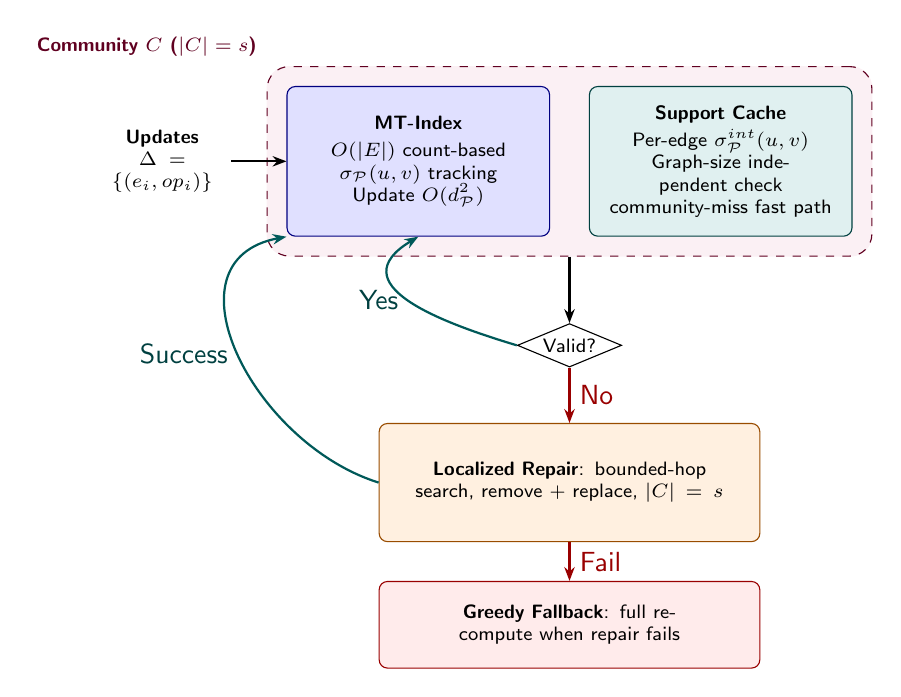
\begin{tikzpicture}[
  font=\sffamily,
  node distance=5pt,
  every node/.style={align=center},
  box/.style={draw, rounded corners=3pt, minimum height=1.3cm, font=\sffamily\scriptsize},
  arr/.style={-{Stealth[length=5pt]}, thick},
  yesarr/.style={arr, color=teal!70!black},
  noarr/.style={arr, color=red!60!black},
]

\node[box, fill=blue!12, draw=blue!50!black, minimum height=1.9cm, text width=3.1cm]
  (mtidx) {\textbf{MT-Index}\\[2pt] $O(|E|)$ count-based\\ $\sigma_{\mathcal{P}}(u,v)$ tracking\\ Update $O(d_{\mathcal{P}}^2)$};

\node[box, fill=teal!12, draw=teal!50!black, minimum height=1.9cm, text width=3.1cm, right=14pt of mtidx]
  (cache) {\textbf{Support Cache}\\[2pt] Per-edge $\sigma_{\mathcal{P}}^{int}(u,v)$\\ Graph-size independent check\\ community-miss fast path};

\node[draw, dashed, rounded corners=8pt, draw=purple!50!black,
      fit=(mtidx)(cache), inner sep=7pt,
      label={[font=\sffamily\scriptsize\bfseries, text=purple!50!black]north west:Community $C$ ($|C|=s$)}]
  (community) {};
\begin{scope}[on background layer]
\fill[purple!6, rounded corners=8pt] (community.south west) rectangle (community.north east);
\end{scope}

\node[left=20pt of mtidx, text width=1.5cm, font=\sffamily\scriptsize] (input)
  {\textbf{Updates}\\ $\Delta=\{(e_i,op_i)\}$};
\draw[arr] (input) -- (mtidx);

\node[diamond, draw, aspect=2.4, below=24pt of community, font=\sffamily\scriptsize, inner sep=1pt]
  (valid) {Valid?};
\draw[arr] (community.south -| valid.north) -- (valid.north);

\node[box, fill=orange!12, draw=orange!60!black, below=20pt of valid, minimum height=1.5cm, text width=4.6cm]
  (repair) {\textbf{Localized Repair}: bounded-hop search, remove + replace, $|C|=s$};
\draw[noarr] (valid.south) -- (repair.north) node[pos=0.5, right, text=red!60!black] {No};

\node[box, fill=red!8, draw=red!60!black, below=14pt of repair, minimum height=1.1cm, text width=4.6cm]
  (fallback) {\textbf{Greedy Fallback}: full recompute when repair fails};
\draw[noarr] (repair) -- (fallback) node[pos=0.5, right, text=red!60!black] {Fail};

\draw[yesarr] (valid.west) .. controls +(-1.0,0.3) and +(-1.0,-0.6) .. (mtidx.south)
  node[pos=0.5, left, text=teal!50!black] {Yes};
\draw[yesarr] (repair.west) .. controls +(-1.6,0.5) and +(-1.6,-0.3) .. (mtidx.south west)
  node[pos=0.5, left, text=teal!50!black] {Success};

\end{tikzpicture}}
\caption{System architecture of \DynaSCSH. Projected source-edge updates enter the \mtindex\ (global meta-path triangle tracking), which feeds the Internal Support Cache inside the maintained community $C$. The validity check (diamond) routes updates: valid communities return immediately to the \mtindex\ (\emph{Yes}, graph-size independent fast path); violations (\emph{No}) trigger Localized Repair, which restores $C$ on success or falls back to fixed-query greedy recomputation (\emph{Fail}) when no bounded-hop replacement exists.}
\Description{Architecture diagram showing update flow from projected source-edge updates through MT-Index, support cache, validity check, localized repair, and greedy fallback.}
\label{fig:architecture}
\end{figure}

\subsection[Meta-Path Triangle Index]{Meta-Path Triangle Index (\mtindex)}

The \mtindex is a count-based index storing, for each edge $(u,v)$, the number of meta-path triangles in which it participates: $\sigma_{\mathcal{P}}(u,v)$. Unlike naive explicit-storage approaches that materialize triangle node tuples at $O(|E|\cdot d_{\max}^2)$ memory cost, the \mtindex stores only integer counts---$O(|E|)$ memory.

\textbf{Construction.} For each node of type $T_1$ (the source type of $\mathcal{P}$), we enumerate its $\mathcal{P}$-neighbors and check triangle closure among pairs of neighbors. Each undirected edge is incremented exactly once per triangle, ensuring exact 1:1 counting (the total edge support sum is always divisible by 3).

\textbf{Update.} For an insertion $(u,v)$, \mtindex enumerates common $\mathcal{P}$-neighbors and increments the three edge supports of each new triangle. For a deletion, it enumerates the witnesses before removing $(u,v)$ and decrements the same three supports. The update cost is $O(d_{\mathcal{P}}(u)d_{\mathcal{P}}(v))$, proportional to endpoint meta-path degrees. Raw HIN relation updates that change many projected source edges require projection refresh or index rebuild; they are outside the per-source-edge complexity claim.

\textbf{Cascading collapse.} During $k$-truss peeling, when an edge is removed we must decrement the support of co-triangle edges. The \mtindex resolves these co-triangle edges on-demand via the \texttt{find\_co\_triangle\_edges} procedure, avoiding the need to pre-materialize triangle adjacency structures.

\subsection{Internal Support Cache}

The $(k,\mathcal{P})$-truss requires that each community edge has at least $k$ \emph{internal} triangles---triangles whose three nodes all lie within the community. Computing this from scratch requires $O(|C|^2 \cdot d_{\mathcal{P}}^2)$ time per validity check, which is prohibitive for high-velocity streams.

The internal support cache is a dictionary mapping each community edge $(u,v)$ to its \emph{internal} support count: the number of nodes $w \in C$ such that $(u,v,w)$ form a meta-path triangle. The cache is built once during community initialization ($O(|C|^2)$) and then updated incrementally:

\begin{itemize}
\item \textbf{Edge insertion in community}: The new edge's internal support is computed on-demand. Existing edges' support is unaffected (monotonicity---insertions only increase global support, so internal support cannot decrease).
\item \textbf{Edge deletion in community}: The deleted edge is removed from the cache. For each triangle $(u,v,w)$ that included the deleted edge, the internal support of edges $(u,w)$ and $(v,w)$ is decremented by 1.
\end{itemize}

\textbf{Graph-size independent validity check.} After any update, checking whether the community remains valid reduces to iterating over the cached dictionary and testing whether any edge has support $< k$, followed by a triangle-connectivity check when a community edge is deleted. This is $O(s^3)$ in the worst case for a size bound $s$, but it is independent of $|V|$ and $|E|$ and completes in microseconds for the small communities used in interactive search ($s \leq 20$ in our experiments).

\textbf{Monotonicity optimization.} Edge insertions \emph{monotonically increase} the global triangle support of all edges. Since the internal support of a community edge cannot decrease after an insertion, a valid community remains valid. \DynaSCSH exploits this by returning immediately on insertion---no validity check, no repair.

\subsection{Incremental Update Protocol}

Algorithm~1 formalizes the update protocol.

\begin{algorithm}[t]
\caption{Incremental Update Protocol for \DynaSCSH}
\label{alg:update}
\begin{algorithmic}[1]
\STATE \textbf{On edge insertion} $(u,v)$:
\STATE \quad $\mtindex.\text{add\_edge}(u,v)$
\STATE \quad \textbf{if} $C = \emptyset$ \textbf{then} return \textsc{FullRecompute}()
\STATE \quad \textbf{if} $u \in C \land v \in C$ \textbf{then} refresh internal support cache
\STATE \quad return $C$ \quad // monotonicity guarantees validity
\STATE \textbf{On edge deletion} $(u,v)$:
\STATE \quad $\mtindex.\text{remove\_edge}(u,v)$
\STATE \quad \textbf{if} $u \notin C \lor v \notin C$ \textbf{then} return $C$ \quad // community-miss fast path
\STATE \quad refresh internal support cache for $C$
\STATE \quad $\mathcal{V} \leftarrow$ \{edges with support $< k$\}
\STATE \quad \textbf{if} $\mathcal{V} = \emptyset$ \textbf{then} return $C$
\STATE \quad \textbf{if} \textsc{LocalizedRepair}($\mathcal{V}$)
\STATE \quad\quad \textbf{then} return repaired $C$
\STATE \quad \textbf{else} return \textsc{FullRecompute}()
\end{algorithmic}
\end{algorithm}

\subsection{Localized Repair}

When community edges violate the $k$-truss condition after a deletion, \DynaSCSH attempts localized repair before falling back to full recomputation. The repair procedure:

\begin{enumerate}
\item Identifies nodes incident to the most violating edges, excluding the original query node from removal.
\item Removes the worst-offending non-query node and searches for a replacement node within $h$ BFS hops of the affected region.
\item Accepts the replacement only if the resulting node set has size $s$, contains the original query node, satisfies internal support $\geq k$ for every induced edge, and remains triangle-connected.
\item If the candidate fails validation, backtracks and tries the next offending node.
\item If no single-node repair succeeds, triggers full recomputation via the same fixed-query greedy heuristic used by the static baseline.
\end{enumerate}

The hop limit $h$ controls the repair search radius and the size of the candidate set; it affects latency but not correctness, because every candidate is fully validated before it can be returned.

\textbf{Correctness invariants.} Three invariants are maintained at every return point. (I1) \emph{Support invariant}: the internal support cache equals $\sigma_{\mathcal{P}}^{int}(u,v)$ for every induced community edge $(u,v)$, counted strictly over $\mathcal{G}[C]$. Insertions refresh the cache when they touch $C$; deletions that touch $C$ rebuild the cache exactly because $s$ is small. (I2) \emph{Query-size invariant}: any returned community contains the original query node $q$ and has $|C|=s$. Localized repair excludes $q$ from removal and accepts only exact-size replacements; fallback recomputation is called with the stored query node rather than an arbitrary surviving node. (I3) \emph{Truss-validity invariant}: any returned community satisfies both internal support and triangle connectivity. This is not inferred from hop locality. The implementation explicitly recomputes internal supports for the candidate node set and runs a triangle-connectivity check before accepting a repair. If validation fails, the candidate is rejected and the algorithm either tries another local repair or invokes \textsc{FullRecompute}. Thus localized repair is an optimization path, not a source of weakened correctness.

\subsection{Complexity Analysis}

\begin{table}[htbp]
\centering
\caption{Per-update time complexity under projected source-edge updates. $d_{\mathcal{P}}$ denotes meta-path degree. The recompute row reflects the polynomial-time greedy heuristic; the NP-hard exact B\&B worst-case is exponential.}
\label{tab:complexity}
\resizebox{\columnwidth}{!}{%
\begin{tabular}{c c c}
\toprule
Scenario & Complexity & Typical \\
\midrule
Insertion (community miss) & $O(d_{\mathcal{P}}^2)$ index update & $<1$~ms \\
Insertion (community hit) & $O(d_{\mathcal{P}}^2 + s^3)$ & $<1$~ms \\
Deletion (community miss) & $O(d_{\mathcal{P}}^2)$ index update & $<1$~ms \\
Deletion (comm. hit, repair ok) & $O(d_{\mathcal{P}}^2 + s^3 + |\mathcal{B}_h|s^3)$ & 1--10~ms \\
Deletion (repair fail) & repair cost $+$ greedy recompute & 390--950~ms \\
\bottomrule
\end{tabular}%
}
\end{table}

Table~\ref{tab:complexity} summarizes per-update complexity. The ``repair fail'' row reflects the polynomial-time greedy heuristic fallback used in our implementation (and in the static practical baseline); the NP-hard exact B\&B would carry exponential worst-case cost. The critical insight is that the dominant path is independent of the full graph size after the \mtindex update: most random projected-edge updates do not touch community edges, while the expensive repair/recompute paths activate mainly under targeted deletions. Here $\mathcal{B}_h$ is the bounded-hop candidate set explored by local repair.

\section{Experiments}

We evaluate \DynaSCSH across fixed-query synthetic configurations and a separate hybrid benchmark, targeting three questions: (Q1) What is the average-case speedup over static recomputation? (Q2) What happens when deletions force fallback-dominated behavior? (Q3) Does the framework scale to 100K-edge graph sizes?

\subsection{Experimental Setup}
\label{sec:setup}

\textbf{Evaluation settings.} We report two evidence-backed graph settings:
\begin{enumerate}
\item \textbf{Synthetic DBLP}: compact DBLP-like network with planted dense groups, used for all 22 fixed-query configurations.
\item \textbf{Hybrid} (26,850 nodes, 128,227 edges): 40 dense planted communities injected into the real 26K-node MAGNN DBLP graph~\cite{fu2020magnn}. This setting tests whether the \mtindex and repair machinery remain practical on a 100K-edge topology with guaranteed valid communities.
\end{enumerate}

\textbf{Update model.} The implementation maintains communities over the source-type graph induced by a symmetric meta-path, e.g., Author--Author projected edges under APA. This matches the edge set on which $(k,\mathcal{P})$-truss support is defined. Raw HIN relation updates such as Author--Paper insertions can change many projected source edges; supporting them incrementally requires a projection-refresh layer and is outside the per-source-edge complexity claim.

\textbf{Baselines and internal fairness.} We compare against \textbf{Static Recompute}: greedy heuristic community search from scratch after each update, equivalent to Zhang et al.'s polynomial-time baseline~\cite{zhang2025scsh}. Both the static baseline and \DynaSCSH's fallback path preserve the \emph{same original query node} throughout an update stream. This fixed-query condition is essential: using an endpoint of the latest update as the recomputation query can create artificial Jaccard divergence and invalid quality comparisons. Under the fixed-query design, the reported speedup measures the benefit of incremental maintenance against the exact algorithm the system itself would run if incrementality were disabled. Using exact B\&B as the baseline would compare a polynomial-time incremental method against an exponential-time oracle, mixing the effect of algorithmic choice with the effect of incrementality. As \DynaSCSH is the first dynamic approach for \emph{size-constrained} HIN communities, no existing dynamic baselines (e.g., CS-DAHIN~\cite{song2024tkde}) can enforce the exact cardinality constraint $|C|=s$; they produce communities of variable size, and post-hoc truncation violates the $(k,\mathcal{P})$-truss condition.

\textbf{Metrics.} (1) \textbf{Speedup}: ratio of static baseline latency to \DynaSCSH latency; (2) \textbf{\qratio}: $\text{score}_{\text{DynaSCSH}} / \text{score}_{\text{static}}$---measures relative community cohesiveness; (3) \textbf{Jaccard similarity}: structural overlap between maintained and recomputed communities.

\textbf{Environment.} Python 3.10, networkx 3.4.2, NumPy 2.2.6, single machine (Intel Core i7-13700, 32\,GB DDR5 RAM). All experiments are CPU-only. Each nonempty synthetic run uses 3 query nodes, 500--1,000 updates, and checkpoints every 10\% of the stream. The artifact includes the experiment runner and a post-fix invariant smoke script that checks fixed-query recomputation, \mtindex co-triangle updates, and community validation.

\textbf{Fast-path interpretation.} For projected-edge deletions, the dominant fast path occurs when the deleted edge is not internal to the maintained community. The exact hit rate depends on the community size, graph density, and update distribution; the implementation therefore checks this condition at runtime rather than assuming a fixed percentage.

\subsection{Average-Case Efficiency (Random Streams)}

Table~\ref{tab:main_results} reports results on the small synthetic benchmark using the fixed-query implementation where both \DynaSCSH's fallback and the static baseline recompute from the same original query node.

\begin{table}[htbp]
\centering
\caption{Representative synthetic DBLP results under the fixed-query baseline. Insertion streams preserve community identity; deletion and mixed streams show natural divergence.}
\label{tab:main_results}
\resizebox{\columnwidth}{!}{%
\begin{tabular}{c c c c c}
\toprule
Run & Type & Speedup & Jaccard & \qratio \\
\midrule
A1 & insertion & 3,478$\times$ & 1.000 & 1.000 \\
A2 & deletion & 3,342$\times$ & 0.362 & 0.887 \\
A3 & mixed & 4,410$\times$ & 0.615 & 0.959 \\
D1 & deletion stress & 1.4$\times$ & 0.544 & 0.916 \\
\midrule
A7\_s5 & insertion, $s$=5 & 3,916$\times$ & 1.000 & 1.000 \\
A7\_s20 & insertion, $s$=20 & 3,569$\times$ & 1.000 & 1.004 \\
\midrule
A8\_k3 & insertion, $k$=3 & 3,847$\times$ & 1.000 & 1.000 \\
A8\_k6 & insertion, $k$=6 & 3,931$\times$ & 1.000 & 1.000 \\
\bottomrule
\end{tabular}%
}
\end{table}

\textbf{Insertion streams.} Across all 17 insertion configurations, \DynaSCSH maintains exact community identity (Jaccard=1.000 in every run). The average \qratio is 1.000, with per-run rounded values from 1.000 to 1.004; the small values above 1.000 arise from greedy tie-breaking, not a claimed quality improvement. Average speedup is 3,824$\times$ (max 4,130$\times$). With a fixed query node, both \DynaSCSH and the static baseline converge to the same greedy community, and edge insertions---which monotonically increase support---do not invalidate the community.

\textbf{Deletion streams.} Three deletion configurations (A2, B2, D1) reveal the tension between community continuity and per-snapshot optimality. Random deletions (A2, B2) achieve Jaccard 0.362 and \qratio 0.887 at 3,200--3,300$\times$ speedup. Across all three deletion configurations, average speedup is 2,188$\times$, Jaccard spans 0.36--0.54, and \qratio spans 0.89--0.92. \DynaSCSH prioritizes valid, low-latency continuity: the maintained community evolves incrementally, while the static baseline can recompute a different greedy community on each snapshot. The D1 deletion stress run drops to 1.4$\times$ speedup, showing the fallback-dominated lower bound when local maintenance does not stay on the fast path.

\subsection{Fallback-Dominated Deletion Behavior}

The D1 deletion stress run is the clearest evidence for the lower-bound behavior of the framework. Unlike insertion streams, deletion can invalidate internal support and force the algorithm to refresh the support cache, attempt repair, or fall back to fixed-query greedy recomputation. In D1, the average dynamic latency rises to 286.3~ms while the static baseline averages 408.5~ms, yielding only 1.4$\times$ speedup. The maintained community remains valid under the invariant checker, but the benefit of incrementality largely disappears because the update stream repeatedly leaves the cheap path.

\textbf{Q2 answered:} Deletions are update-pattern dependent. \DynaSCSH is extremely fast when validation remains local, but strict invariant checking deliberately sacrifices speed and invokes recomputation when local repair cannot certify support, size, query containment, and triangle connectivity.

\subsection{Community Quality Tracking}

A key lesson from the revised artifact is that quality must be interpreted under a fixed-query protocol. Earlier experiments reported low Jaccard similarity between maintained and recomputed communities, but fixed-query post-fix smoke validation shows that insertion streams can preserve both structure and score exactly. We therefore report Jaccard as a diagnostic rather than a primary quality claim.

The deletion results show path dependence in the opposite direction: static from-scratch greedy search can recover a different community, while \DynaSCSH preserves a valid incumbent until repair or fallback is required. This can reduce \qratio when the maintained community loses support and no bounded-hop repair is available. The revised claim is therefore narrow: dynamic maintenance creates a speed-quality trade-off controlled by validation and fallback, rather than a quality guarantee.

This phenomenon arises from the path-dependence of combinatorial search in dense graphs. When many valid size-constrained communities exist, incremental repair and static greedy recomputation may converge to different valid solutions. The revised artifact controls this comparison by preserving the original query node and by validating any locally repaired community before it is returned.

\subsection{Real-World Scalability: Beyond Latency}

\begin{figure}[htbp]
\centering
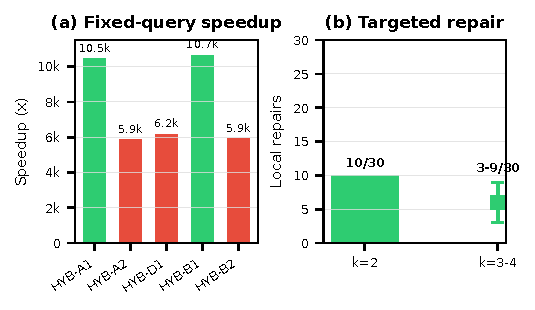
\includegraphics[width=\columnwidth]{figures/fig_hybrid_benchmark.pdf}
\caption{Hybrid benchmark results: 40 planted communities on 26K-node real DBLP. At $k$=2, \DynaSCSH repairs 10/30 targeted community-edge deletions locally with 0 recomputes.}
\Description{Hybrid benchmark plot showing fixed-query random-stream speedups and targeted local-repair success on a 26K-node planted DBLP graph.}
\label{fig:hybrid}
\end{figure}

We evaluate \DynaSCSH on the hybrid graph (26,850 nodes, 128,227 edges)---the Planted Community Benchmark combining real DBLP topology with 40 dense planted communities---under the fixed-query implementation to answer: (1) does the framework scale to 100K-edge graphs, and (2) how does incremental maintenance behave at realistic scale?

\textbf{Scaling of the speedup advantage.} Table~\ref{tab:hybrid} reports results across five experiment configurations. The hybrid runs maintain sub-millisecond dynamic latency on 128K edges. Static recomputation averages $\approx$900--944~ms, while DynaSCSH's incremental path remains below 0.16~ms on average. On insertion streams, \DynaSCSH achieves perfect community identity (Jaccard=1.000, \qratio=1.000, speedup 10,500--10,700$\times$). On deletion streams, community identity is preserved (Jaccard=1.000) with aggregate \qratio 0.933--0.934 and speedup 5,900--6,200$\times$.

\begin{table}[htbp]
\centering
\caption{Hybrid graph results under fixed-query implementation (26,850 nodes, 128,227 edges).}
\label{tab:hybrid}
\resizebox{\columnwidth}{!}{%
\begin{tabular}{c c c c c c}
\toprule
Run & $k$ & Type & Speedup & Jaccard & \qratio \\
\midrule
HYB-A1 & 2 & insertion & 10,451$\times$ & 1.000 & 1.000 \\
HYB-A2 & 2 & deletion & 5,853$\times$ & 1.000 & 0.934 \\
HYB-D1 & 3 & deletion & 6,160$\times$ & 1.000 & 0.933 \\
HYB-B1 & 2 & insertion & 10,654$\times$ & 1.000 & 1.000 \\
HYB-B2 & 2 & deletion & 5,921$\times$ & 1.000 & 0.934 \\
\bottomrule
\end{tabular}%
}
\end{table}

\textbf{Community continuity under fixed query.} The fixed-query implementation reveals a clean aggregate pattern: insertion streams preserve exact community identity, and the reported hybrid deletion runs also preserve Jaccard=1.000 while showing lower cohesiveness than the static greedy baseline (\qratio 0.933--0.934). Four fallback recomputations are recorded in each hybrid deletion summary, triggered by the strict invariant checker when local repair cannot find a valid replacement.

\textbf{Repair at scale.} To isolate repair performance, we constructed a targeted repair experiment: 30 targeted deletions from community edges at each $k$ level. Table~\ref{tab:hybrid_repair} reports the results. At $k$=2, 10 out of 30 targeted deletions were repaired locally with 0 recomputes---the larger graph provides a richer candidate pool. At higher $k$, stricter truss constraints reduce repair success and increase fallback.

\begin{table}[htbp]
\centering
\caption{Targeted hybrid repair test (30 community-edge deletions per $k$ level).}
\label{tab:hybrid_repair}
\begin{tabular}{c c c c}
\toprule
$k$ & Targeted deletions & Local repairs & Recomps \\
\midrule
2 & 30 & 10 & 0 \\
3--4 & 30 each & 3--9 & 6--9 \\
\bottomrule
\end{tabular}
\end{table}

\textbf{Q3 answered:} \DynaSCSH scales to 128K-edge graphs in the reported hybrid benchmark. Under the fixed-query implementation, insertion streams preserve community identity at 10,000$\times$+ speedup; deletion streams preserve identity with aggregate \qratio near 0.93. Localized repair succeeds at moderate $k$ on sufficiently large graphs. The speedup grows with graph scale because validation and cache maintenance are independent of the full graph size once affected projected-edge supports have been updated, while static recomputation scales with $|E|$.

\subsection{Discussion: The Cost of Dynamism}

\DynaSCSH's design follows a classic database systems principle: optimize for the common case (random updates) while maintaining acceptable behavior under targeted deletions. The three-tier performance profile is: graph-size independent validation for most updates, bounded-hop repair for community-edge hits, and fixed-query greedy recomputation when local validation fails. The hybrid graph experiments further suggest that the speedup advantage is not a constant but a function of graph scale: as graphs grow, the gap between incremental updates and full recomputation widens, making the case for dynamic maintenance increasingly compelling at deployment scale.

\section{Conclusion}

We presented \DynaSCSH, a dynamic framework for maintaining size-constrained $(k,\mathcal{P})$-truss communities over evolving heterogeneous information networks under projected source-edge updates. \DynaSCSH combines three technical contributions: (1) a count-based $O(|E|)$ Meta-Path Triangle Index with $O(d_{\mathcal{P}}^2)$ projected-edge updates, (2) an internal support cache that makes validation independent of the full graph size, and (3) a localized repair mechanism that preserves the original query node and validates internal support plus triangle connectivity before returning a repaired community.

Evaluation across 22 fixed-query synthetic DBLP configurations and a 26,850-node hybrid Planted Community Benchmark demonstrates incremental maintenance under a fixed-query baseline. Insertions preserve identity exactly: Jaccard is 1.000 in all insertion runs, average \qratio is 1.000, and average speedup is 3,824$\times$. Deletions show natural divergence (Jaccard 0.36--0.54, \qratio 0.89--0.92), and the D1 deletion stress run exposes the fallback-dominated lower bound (1.4$\times$ speedup) under strict invariant checking. The hybrid benchmark confirms scalability (random updates $<$1\,ms on 128K edges), 5,900--10,700$\times$ speedup, and repair feasibility (10/30 targeted repairs at $k$=2).

\textbf{Limitations.} \DynaSCSH currently supports a single meta-path, assumes updates over the projected source-type graph, and requires the size bound $s$ to be specified a priori. Raw HIN relation updates require a projection-refresh layer or index rebuild. The fast-path hit rate depends on the community's internal edge count relative to the update distribution and should be measured per deployment. The current local repair heuristic handles one-node replacement with strict $h$-hop BFS candidate search; multi-node repair and stronger replacement ranking are natural next steps. Extending the framework to multiple meta-paths, automatically recommending $s$, and maintaining communities over temporal sliding windows remain open directions.


\bibliographystyle{ACM-Reference-Format}
\bibliography{references}

\end{document}
